
\chapter{Opera}
\label{opera}

\section{Opera post Beethoven}

%%%%%%%%%
%Refer back to previous material but add musical examples
%%%%%%%%%

\section{Ludwig van Beethoven}
\subsection{Fidelio Op.72}
Beethoven's only opera premiered in its final, third version on May 23, 1814.  The overture is bold and symphonic. The action is set in a Spanish state prison near Seville in the 18th century. Leonore, disguised as the male prison guard Fidelio sets about to rescue her husband Florestan (a political prisoner). Act I opens with the unfortunate Marzelline extolling her love for Fidelio whilst avoiding the advances of guard Jaquino.      

\section{Carl Maria von Weber}
\subsection{Der Freisch\"utz} 
Weber (1786-1826) drew upon myth, legend and the supernatural for \textit{Der Freisch\"utz} which premiered in Berlin in 1821. However, many of the scenes are `real' and down to earth. The synopsis is as follows:

\begin{quotation}
Caspar, Max's unsuccessful rival for the love of Agathe, has sold his soul to the devil (who has taken the form of Samiel, the legendary Black Huntsman) and must procure another victim for him. To this end, Caspar persuades Max to make a pact with Samiel for magic bullets that will allow Max to win Agathe's hand when he wins a marksmanship context. The bullets work their magic well, but the last one is controlled by Samiel, who has destined it to kill Agathe. Max uses up three bullets to impress the Prince before the contest begins and has only one left (that guided by Samiel) for the fateful trial. Although Agathe unexpectedly appear in the line of fire as Max shoots, she is protected by an old hermit's magical wreath. The bullet kills Caspar instead, and all ends well. \citep[p640]{grout1996history} 
\end{quotation}

(Act II, scene II is the well known `Wolf's Glen' scene)

\section{Richard Wagner}

\subsection{Tristan und Isolde} 
Wagner was obsessed with mythology and legend. From the \textit{Flying Dutchman} in 1843 through \textit{Tannh\"aser} in 1845 and \textit{Lohengrin} in 1850 his larger operas espoused the romantic vision of love and transfiguration through death. And nowhere more is this true in \textit{Tristan und Isolde} and \textit{Der Ring des Nibelungen}. The Tristan story is hundreds of years old and has Welsh origins.\footnote{Check the history of the legend \textit{Tristan and Iseult} on line for further details} Wagner broke from writing the \textit{Ring} in 1857 to begin \textit{Tristan} and \textit{Die Meistersinger von N\"urnburg}. \textit{Tristan} was completed in 1959. 

Wagner first mentions the idea of the opera in a letter to Liszt in 1854 and it is very possible that this opera was partly inspired by Wagner's infatuation for Mathilde Wesendonck that was unrequited. Partly, because amongst other things that Wagner was doing at that time he sought to create something truly emotional and romantic. Newman \citeyearpar{newman1977wagner} also cites that Wagner was influenced by reading Schopenhauer's philosophy. A written scenario for the opera was produced by April 1957 and a prose sketch  appeared in August 1857. Sketches of numerous key themes are to be found dating back to December 1956 and Wagner details how these themes weighed heavy on his mind as he finished sections of \textit{Siegfried}. Wagner filters down the convoluted back story of legend and produces an opera full of symphonic thought, devoid of excessive narrative and description but laced with passion. 

Leitmotif is dominant in \textit{Tristan} but the opening bars of the opera have become legendary in themselves.

\begin{figure}[H]
\centering
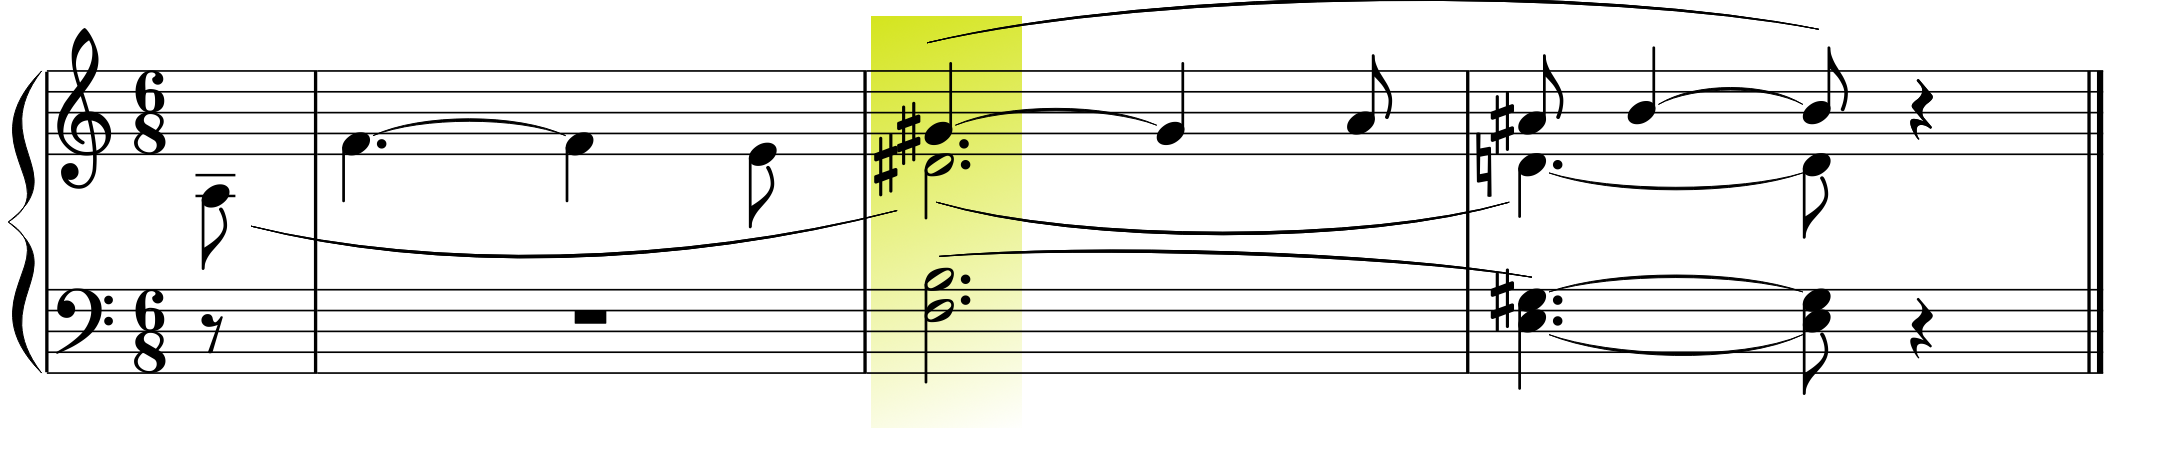
\includegraphics[scale=0.2]{tristanchord}\caption{The opening of \textit{Tristan und Isolde} and the \textit{Tristan chord}}
\label{fig:tristanchord}
\end{figure}

Much has been written about this chord but if we work backwards, we are on a V7 in A minor and the upper parts move by semi-tone steps. The chord itself is an augmented 4th on F plus a perfect 4th, a major third apart. The second half of the phrase (from the G$\sharp$) is known as the Magic theme as it is associated with the passage where Isolde tells of her mother's gift for potion making. 


The rise to the suspension in the first half of figure~\ref{fig:tristannewman2} represents Tristan's anguish and leads directly into the theme associated with the moment in the (back) story where Tristan's glance at Isolde sealed her love and swayed her from slaying him.  

\begin{figure}[h]
\centering
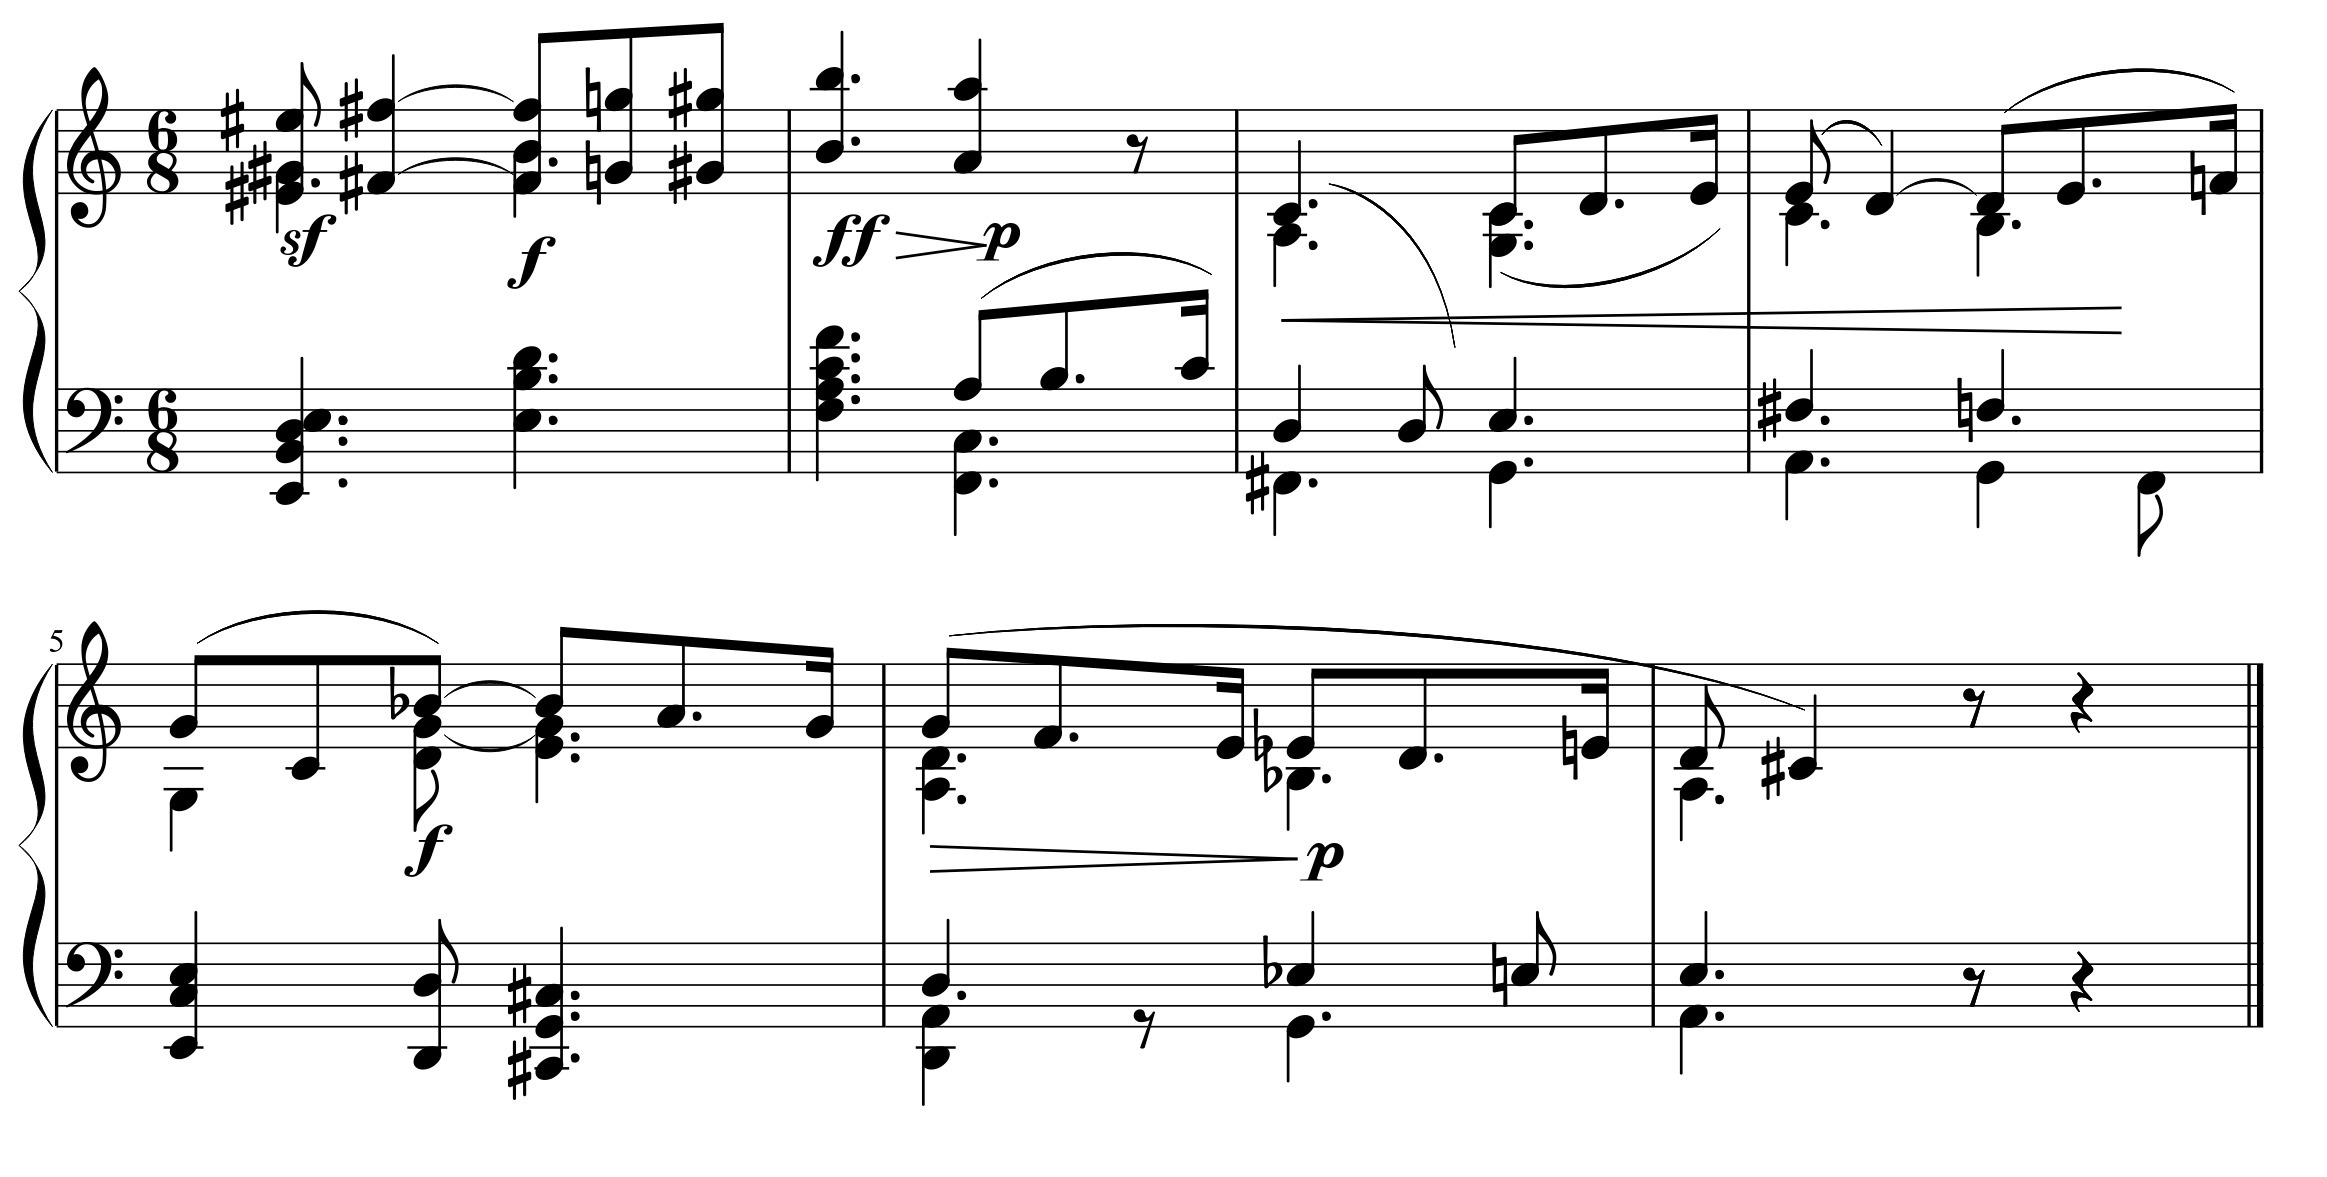
\includegraphics[scale=0.2]{tristannewmantheme2}\caption{`Look' theme}
\label{fig:tristannewman2}
\end{figure}

Much is made of this swelling motive as it moves between orchestral groupings. 

\begin{figure}[H]
\centering
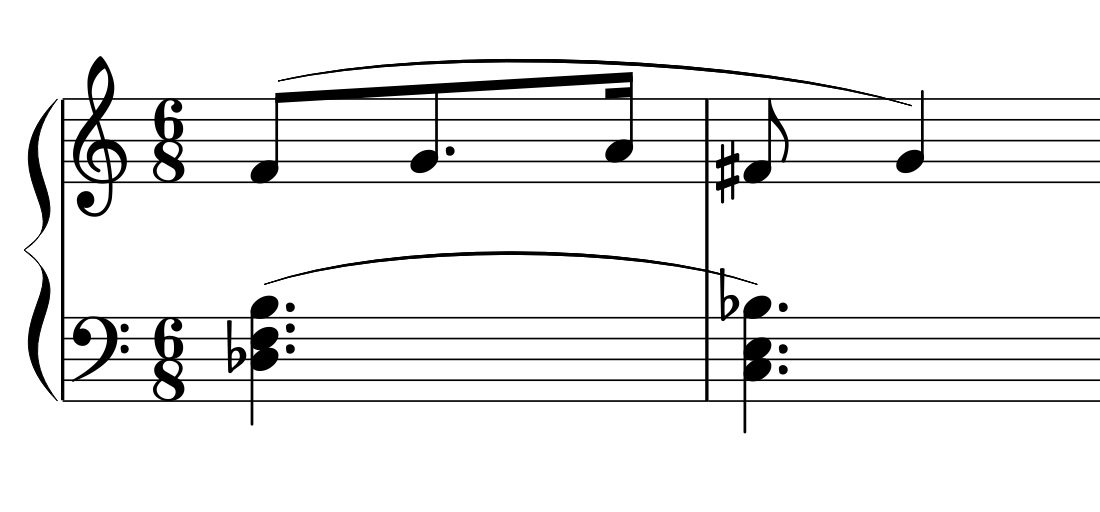
\includegraphics[scale=0.2]{tristannewmantheme4}\caption{Chromatic sequence}
\label{fig:tristanchromaticsequence}
\end{figure}

The prelude relates solely to Act 1 in that it was composed well before the music to Act II and III. The music gets more and more agitated until a final cadence leads to a coda and a repeat of the opening motif. The curtain rises and we are on board a ship heading for the coast of Cornwall. A sailor is singing of an Irish maid which Isolde takes to be a slight at her. As the sailor sings of home a tune more like a Benjamin Britten theme appears. 

\begin{figure}[H]
\centering
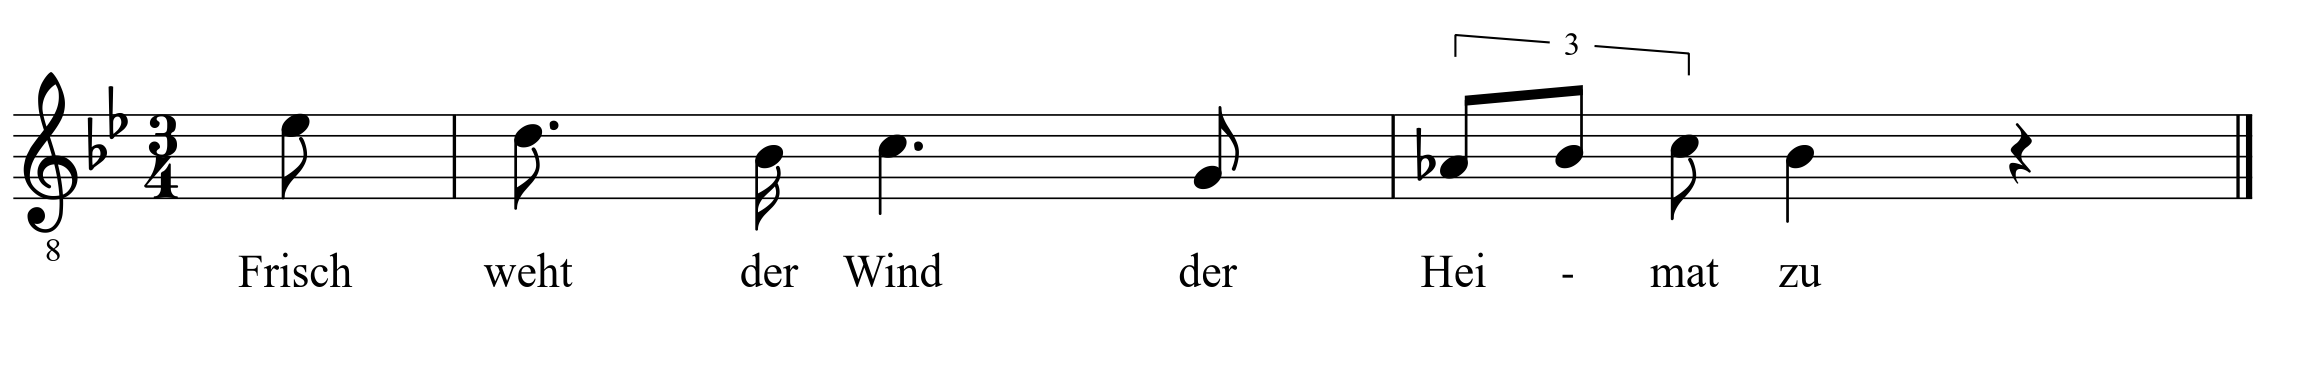
\includegraphics[scale=0.2]{tristannewmantheme9}\caption{Fresh wind to home}
\label{fig:tristanfreshwind}
\end{figure}

Cue much anguish from Isolde and her maid Brangaene. As Isolde sees Tristan she sings the phrase ``Destined to be mine, lost tome; peerless, proud; brave and craven! Death-devoted head! Death-devoted heart!'' - a theme that resonates right till the end of the opera. For Isolde is to the be bride of King Marke.

\begin{figure}[H]
\centering
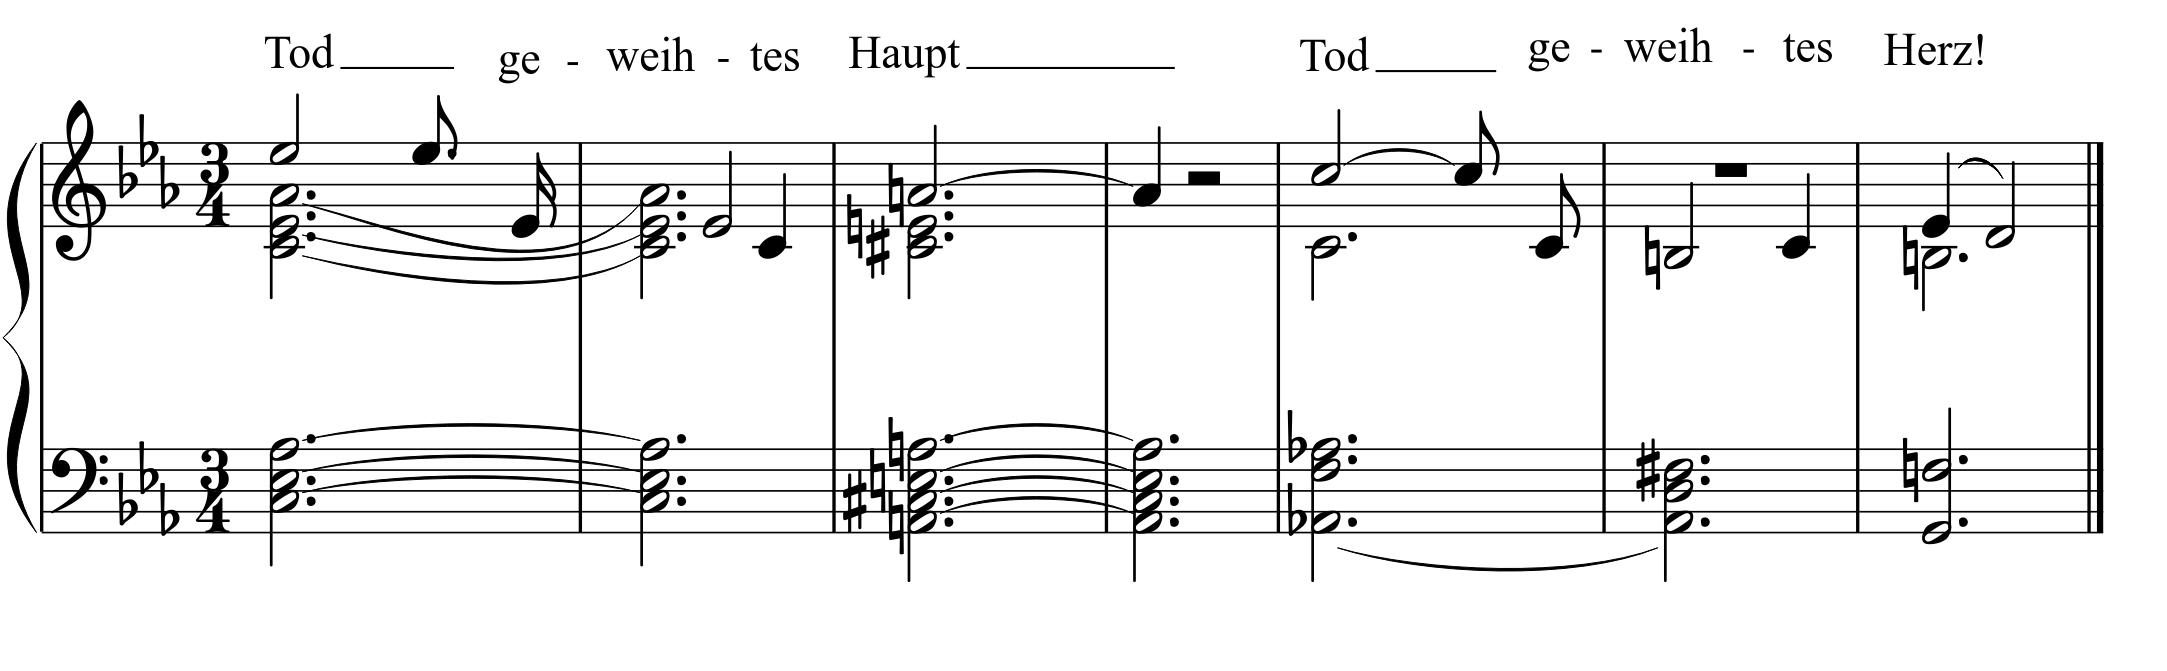
\includegraphics[scale=0.2]{tristannewmantheme13}\caption{Death devoted heart}
\label{fig:tristandeathdevotedheart}
\end{figure}
 
Isolde resolves to kill Tristan with a lethal potion. Brangaene swaps it for a love potion. They both drink it thinking they are to die together - which in act III they do - but instead they seal their love.  

Act II is altogether more boisterous and is where the jealous Melot breaks his loyalty to Tristan as he too is in love with Isolde. The king is hunting and we hear distant horn calls signifying this. Tristan and Isolde are meeting under cover of darkness but Melot and King Marke interrupt them. Everyone's betrayal is laid bare. Melot and Tristan fight and Tristan is mortally wounded. 

Act III sees Tristan gravely ill but returned to his castle by his servant Kurwenal. This act is, like the first, sorrowful in the extreme. Tristan succumbs to his wounds as Isolde arrives by boat. Melot and the king are not far behind in another boat. Kurwenal kills Melot and is himself slain. The king explains that he has in fact followed Isolde to unit her with Tristan. Isolde is reunited with Tristan in death. 

This opera has all the tragedy of Verdi's romantic works but at its heart is redemption and transfiguration through death, something deeply spiritual, something that music seems to embody, something that is not easily described in words.   

\subsection{Further listening} 
\begin{itemize}
\item Richard Strauss: \textit{Death and transfiguration (Tod und Verkl\"arung)}, (1889)
\end{itemize}

\section{Verdi}
Guiseppe Verdi (1813-1901) wrote 26 operas between 1839 and 1893. Libretti for his operas came from (amongst others) the romantic writings of Schiller, Victor Hugo, Byron and of course Shakespeare. 

\begin{itemize}
\item \textit{Macbeth} (premiere 1847 rev. 1865)
\item \textit{Rigoletto} (premiere 1851)
\item \textit{La traviata} (premiere 1853)
\item \textit{Aida} (premiere 1871)
\item \textit{Otello} (premiere 1887)
\item \textit{Falstaff} (premiere 1893)
\end{itemize}

Wagner and Verdi never met and their operas could not be more different. Verdi remains classical throughout the early works, enjoying early success with operas that had at their heart really strong characters. Consequently there are plenty of arias for the stars. 

\subsection{Rigoletto}
Rigoletto is hunchback court jester to the Duke of Mantua and the opening act sees Rigoletto use his spiked 
tongue to get Count Monterone arrested whereupon the Count curses Rigoletto and the Duke. Rigoletto has a 
secret daughter, Gilda. She and the Duke are in love. This drives Rigoletto mad and he hires the assassin 
Sparafucile to murder the Duke. However, as only opera can conceive, Gilda (Rigoletto's daughter) sacrifices 
herself to Sparafucile and the assassin hands over what Rigoletto thinks is the Duke in a sack. Just as 
Rigoletto is about to throw the sack in the river, Rigoletto hears the voice of the Duke singing ``La donna 
\`e mobile'' (woman is flighty). He checks the sack, his daughter revives for one final aria ``V'ho 
ingannato'' (I deceived you) and Rigoletto remembers the curse. 

\begin{itemize}
\item Gilda sings of her love for the Duke: ``Caro nome'' (beloved name), Act I. Scene2. 
\item The Duke sings of the fickle nature of women: ``La donna e mobile'' (Woman are as fickle as feathers in the wind...), Act III. 
\end{itemize}

In addition to highly memorable arias, Verdi was a master of duo/trio/quartet moments.

\subsection{Otello}
Librettist Arrigo Boito showed Verdi the text for \textit{Otello} in 1881. Much is made of how Verdi's publisher, Ricordi encouraged Verdi to get back to writing opera after Verdi, completing Aida had decided to retire. Verdi began work in 1884. As with the lead roles in \textit{Fidelio} the vocal writing for Desdemona, Iago and Otello is challenging. This is grand opera at its most grand. Deception, infidelity, suspicion, love, murder and suicide drive the action. The `um-pah' accompaniments of \textit{Rigoletto} are replaced by full, freely-flowing accompaniments. \textit{Otello} has been sung by Placido Domingo since 1975.

\begin{itemize}
\item Final scene from Act 1 (some 30 minutes into the opera). As Otello and Desdemona kiss ``un bacio ... Otello! ... un bacio''. Read more about the theme with thoroughly thought through harmonic analysis in David Lawton's paper \href{http://www.jstor.org/stable/746411?seq=1#page_scan_tab_contents}{On the ``Bacio'' Theme in \textit{Otello}}. 
\end{itemize}

\section{Romanticism and Puccini: La Boh\`eme}
\begin{itemize}
\item Listen: \url{https://www.youtube.com/watch?v=ntg9vXxAia8}
\item Score: \url{http://imslp.org/wiki/La_boh%C3%A8me_%28Puccini,_Giacomo%29}
\item Reading (not for comment): \url{http://www.pittsburghopera.org/files/file/Study%20Guide%20for%20La%20boheme.pdf}
\end{itemize}

Giacomo Puccini was born into a musical family. Puccini's father was an organist and teacher. Puccini was the fifth of eight children, five girls, three boys. As Puccini learned his trade, his composition teacher introduced him to Verdi's scores (\textit{Rigoletto}, \textit{La traviata}). And from hearing \textit{A\"ida} he began to compose less for the organ. Puccini continued his studies in Milan under the tutelage of Antonio Bazzini beginning in 1880, also with Amilcare Ponchielli. He was joined in Milan by Pietro Mascagni, composer of \textit{Cavalleria Rusticana} (1890), an opera that started the \textit{Verismo} tradition (emphasis upon realism). In 1883 Puccini composed a ten minute orchestral piece, \textit{Capriccio Sinfonico}. Already operatic in nature; dramatic and poignant, one  can hear the beginnings of his phrase structure, the mood swings and the swirling, haunting melodies. The whole work sounds like an introduction and in a way, it is perhaps an overture to larger things. And then all of a sudden we hear the opening of \textit{La Boheme}. 

Just as `getting signed' today is key to success, so it was back then and the two main publishers were Ricordi and Lucca. After two less well known pieces \textit{Le villi} and \textit{Edgar} with libretti by Fernando Fontana, Ricordi commissioned new work and Puccini went through librettist after librettist. It seems Puccini was very picky about who he worked with eventually siding with Giuseppe Giacosa and Luigi Illica. This opera was \textit{Manon Lescaut}. It is interesting to note that Illica and Giacosa were to remain faithful to Puccini for future successful operas. \textit{Manon Lescaut} was completed in 1892 after three years hard work. Immediately it has signature tenor lines and languorous phrasing. Recitative and Aria have disappeared as has a post-Verdi accompanimental style. 

The success of \textit{Manon Lescaut} now set Puccini fair financially. 

\textit{La boh\`eme} comes from Henri M\"urger's Sc\`enes de la vie de boh\`eme. Bohemianism is associated with carefree, gypsy-like lifestyle. There is a relatively intense history pertaining to the emergence of Puccini's version. It seems composers and publishers were all scrambling to the same story. Moreover, the libretto's gestation was lengthy and revised many times. Once the libretto was in good shape, Puccini worked on the score: 1895 saw the completion of the music. The premiere was set for Teatro Regiio, Turin; date 1st February 1896. Despite recommendations for conductors from Puccini, Ricodi selected young conductor Auturo Toscanini.

To top it all, \textit{La boh\`eme} received mixed reviews. 

\subsection{Synopsis}
The Opera is set in the Latin Quarter of Paris around 1830. Four artists are living a poor life. Rodolfo (poet), Marcello (painter), Schaunard (musician) and Colline (philosopher). They are ``Bohemians'', penniless but passionate about life. It's Christmas Eve and three of the men leave the flat to go to the cafe, leaving Rodolfo behind. Enter Mimi, frail, delicate (and ill) to ask for a candle. Love lights up the room. They eventually join the group at the cafe along with Musetta who, accompanied by her much older admirer Alcindoro tempts her ex, Marcello to fall in love with Musetta again. 

A month later. Mimi finds Marcello to tell him that Rudolfo, in a fit of jealousy has left her. When Marcello questions Rodolofo, he explains his departure was due to the fact he can not support her as she is dying (of consumption - TB). Mimi overhears this conversation but they meet and love, once again endures. Marcello and Musetta - now living together - also argue. 

In the fourth act, Marcello and Rudolfo are lamenting love. They are both separated from their loved ones. Schaunard and Colline try to brighten the atmosphere but the merriment is arrested when Musetta arrives with a dying Mimi. The friends go off to search for a doctor leaving Rudolfo and Mimi together. 

\subsection{What makes La Boh\`eme ground-breaking?}
Look at a review from critic of the time Eduard Hanslick (1825-1904)
\begin{quotation}
The few earlier operas that deal seriously with affairs between wanton courtesans and weak youths (\textit{La Traviata, Camen}, and most recently \textit{Manon}) have at least dressed them in picturesque national or historic garb, or set them in romantic surroundings and thus raised them out of the lowest regions of everyday wretchedness. With \textit{La Boh\`eme} our composers take the last step towards the naked, prosaic dissoluteness of our time: heroes in loud-checked trousers, gaudy ties and crumpled felt hats, cigarette butts in their mouths, their companions in bonnets and scanty shawls. This is new, a sensational break with the last romantic and artistic traditions of opera.
\end{quotation}

There's a new, more visceral depiction of everyday life. But amidst the mundane there are moments of pure poetry. In particular note the difference between the words of Mimi when she says, `actually my name is Lucia'. 

\subsection{Musical details}

The opening bravura theme comes from the earlier \textit{Capriccio Sinfonico}. 

\begin{figure}[H]
\centering
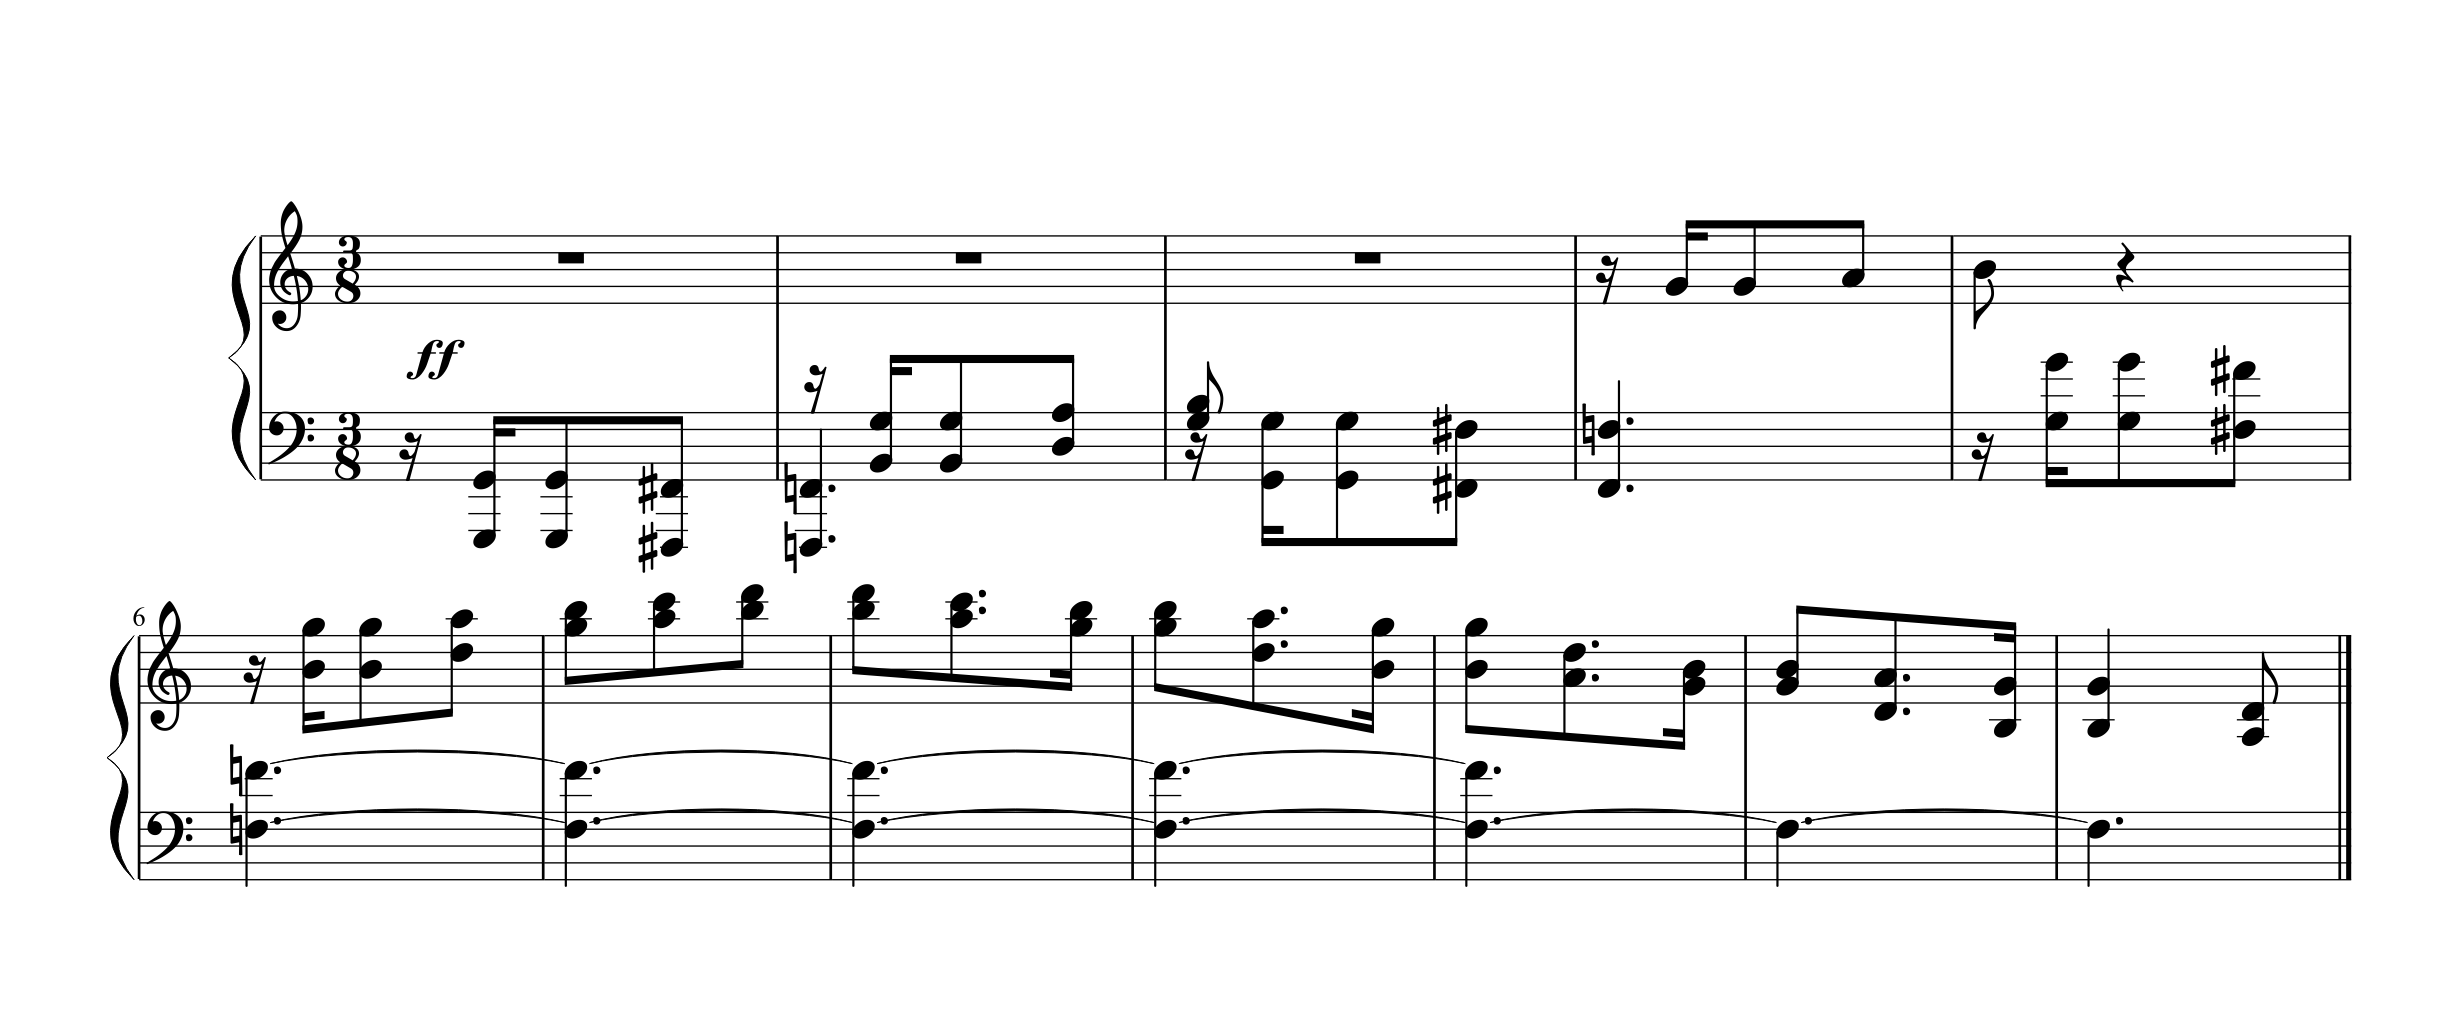
\includegraphics[scale=0.2]{boheme1}\caption{La Boh\`eme opening moments}
\label{fig:boheme1}
\end{figure}

Rodolfo's theme is a plaintive call swaying through high notes.

\begin{figure}[H]
\centering
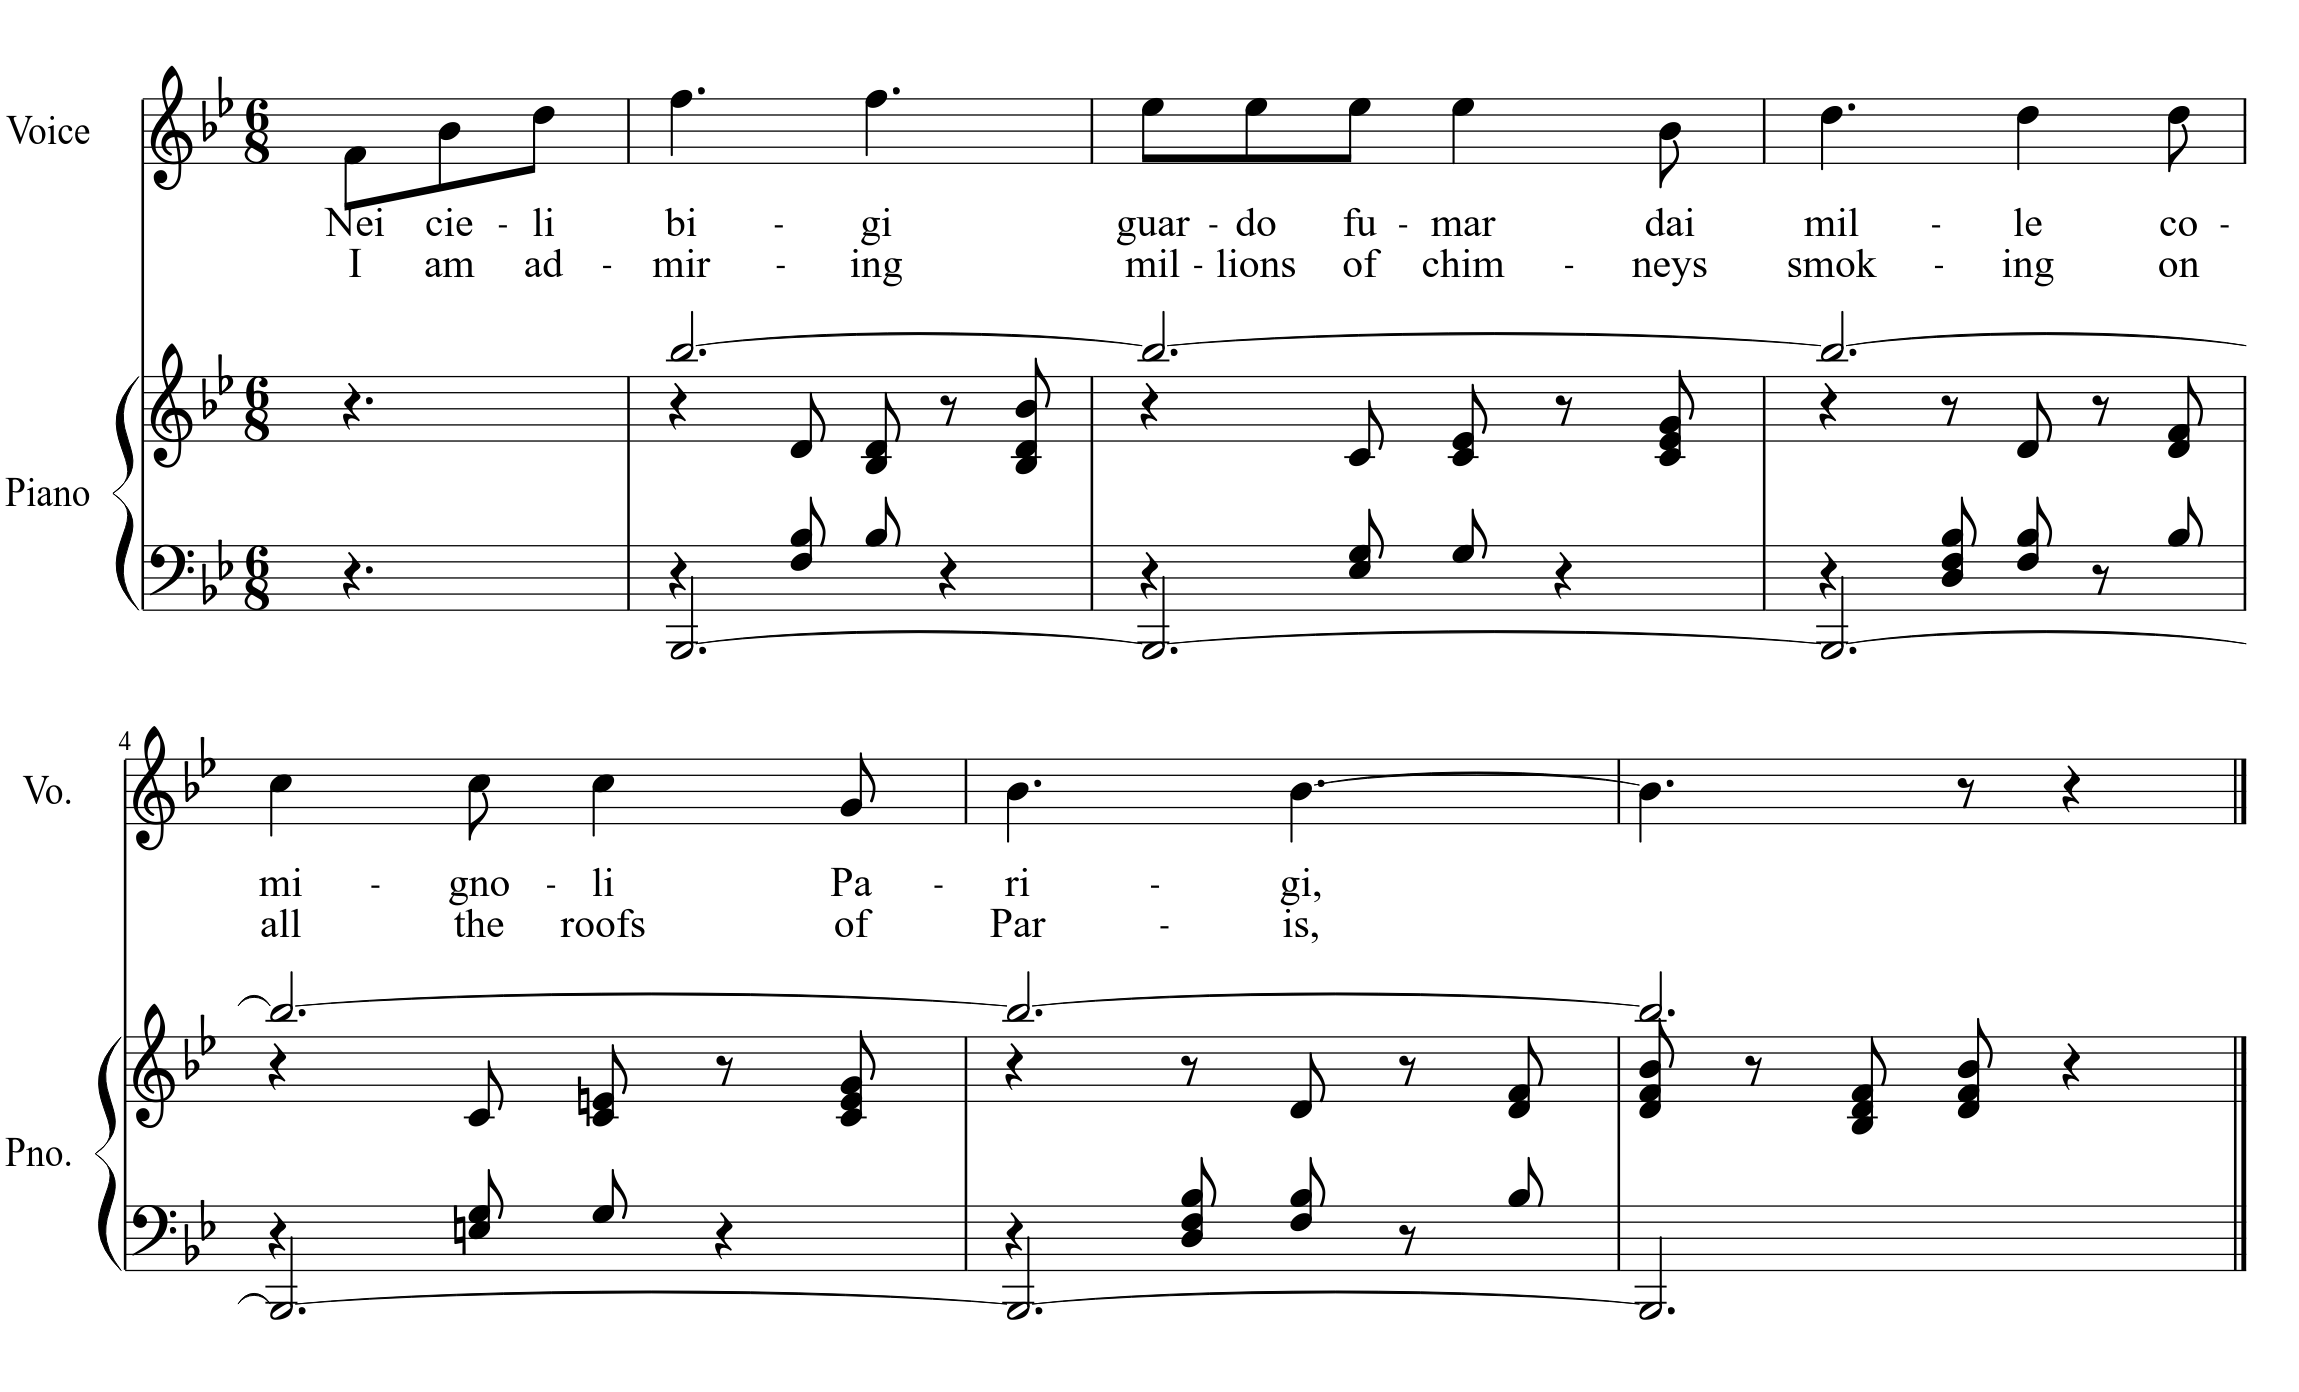
\includegraphics[scale=0.2]{rodolfotheme}\caption{Rodolfo's theme}
\label{fig:rodolfotheme}
\end{figure}
 
The themes are simple but poignant. Note Rodolfo's melody as he and Mimi search for the lost key. This tune could not be easier to remember but its falling (and subsequent climb-fall repeats) represents their forlorn love. 

\begin{figure}[H]
\centering
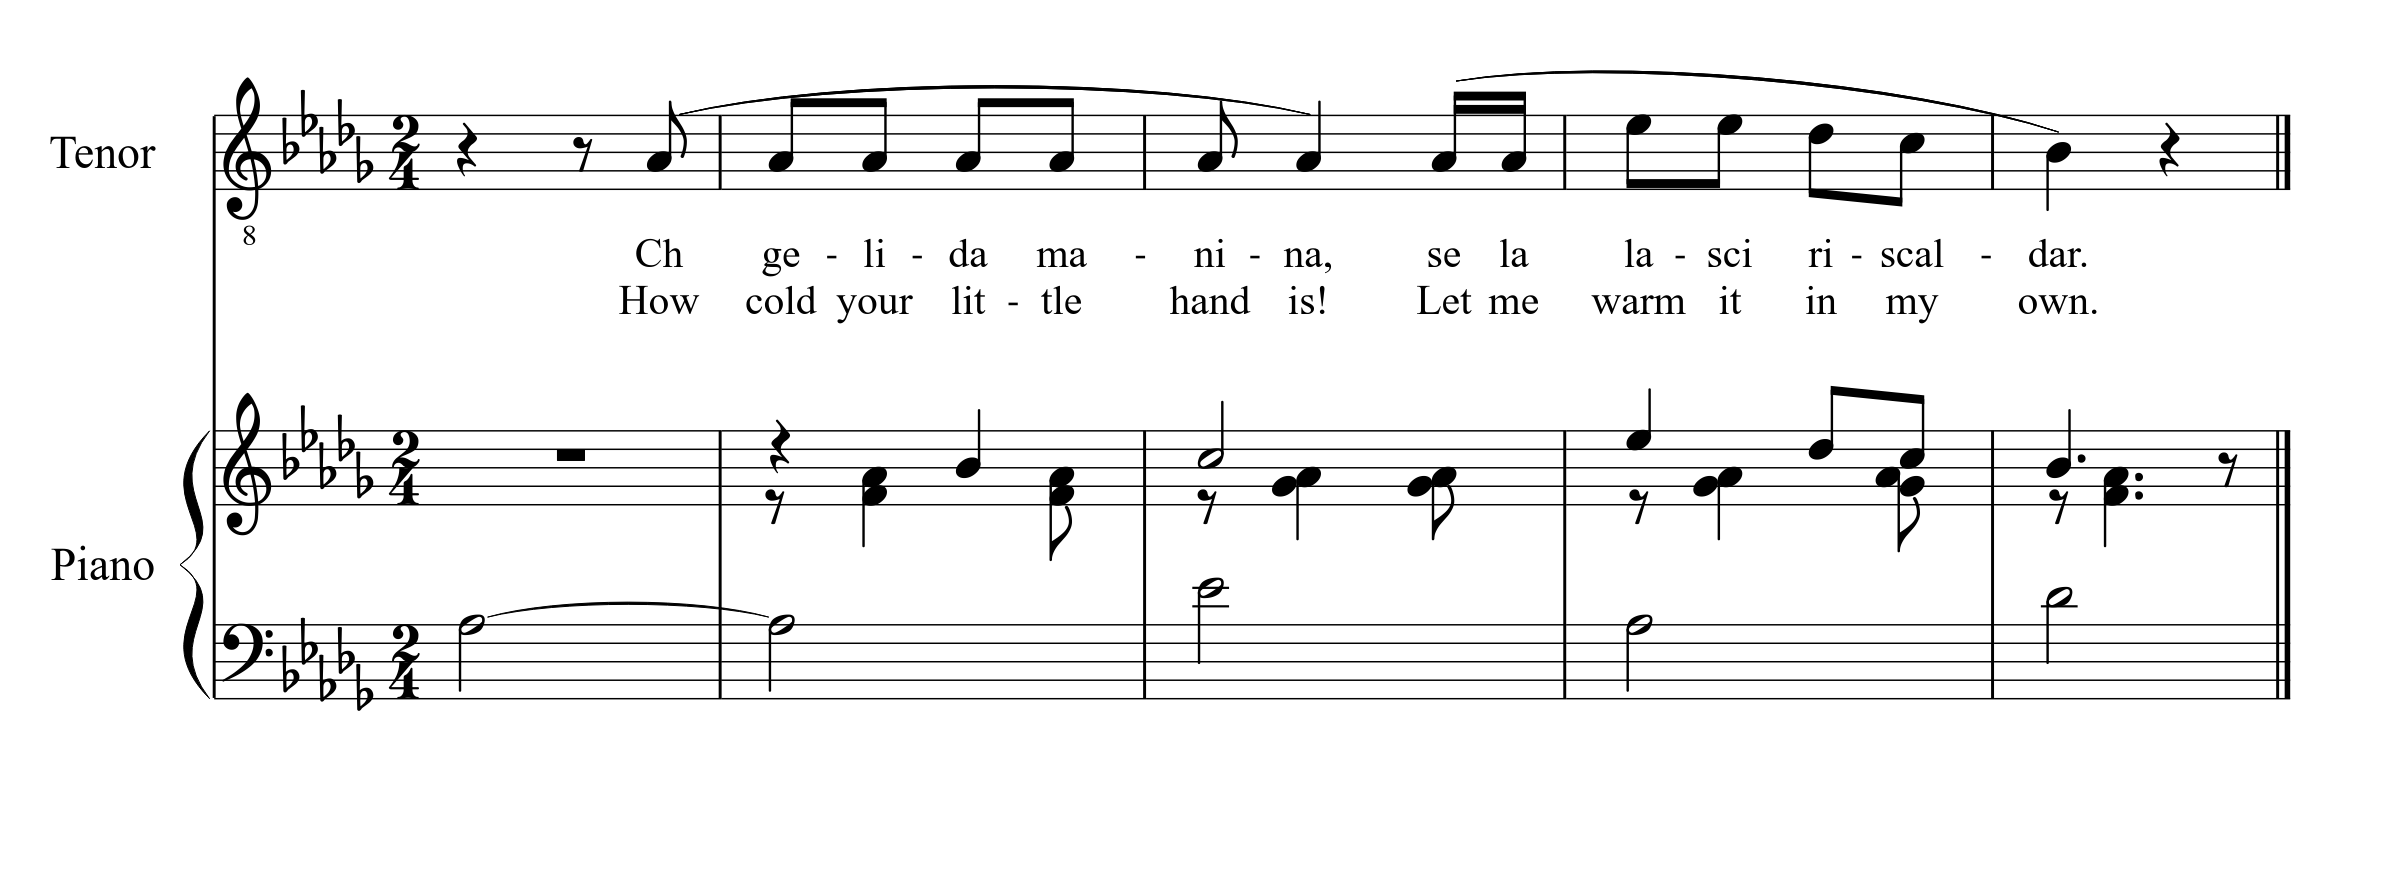
\includegraphics[scale=0.2]{rodolfokey}\caption{Rodolfo's key theme}
\label{fig:rodolfokey}
\end{figure}

Act II is the `Quatier Latin' and the boisterous atmosphere is represented by bristling parallel chords. 

\begin{figure}[H]
\centering
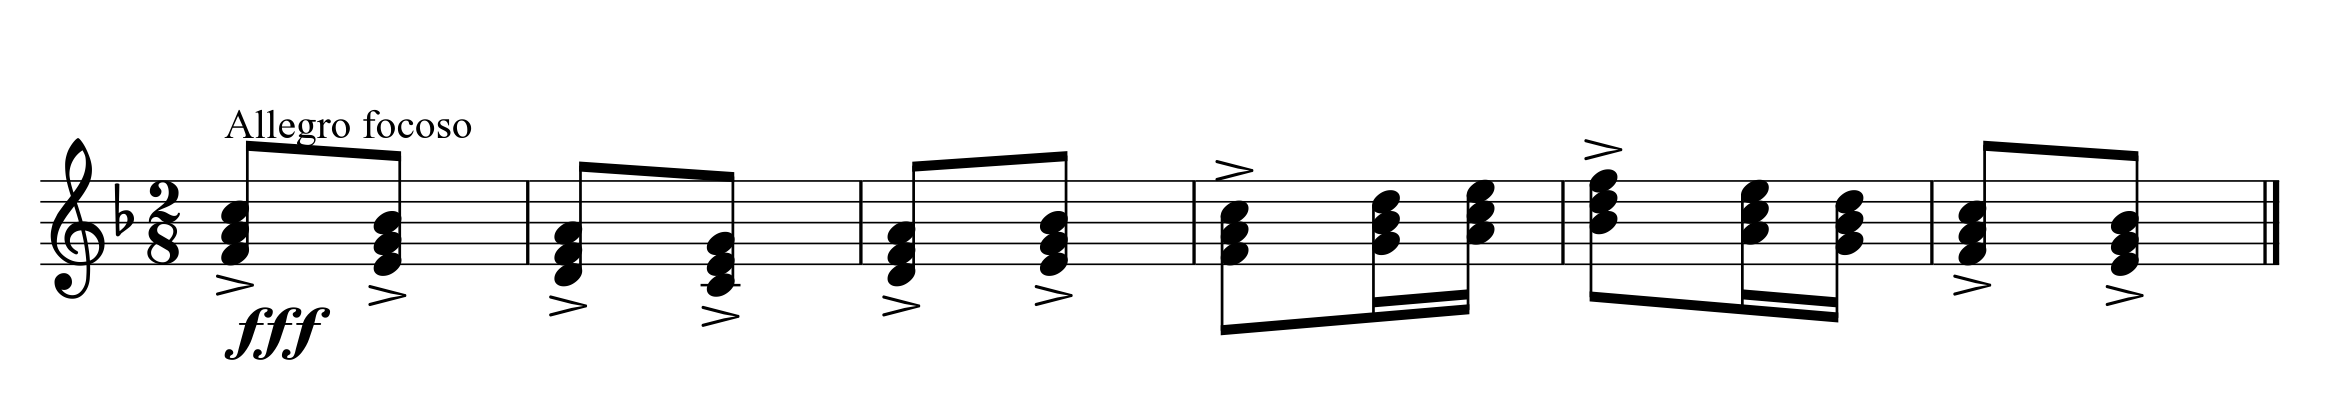
\includegraphics[scale=0.2]{quatierlatin}\caption{Quatier Latin opening}
\label{fig:quatierlatin}
\end{figure}

To add to the reality we see the arrival of toy maker Parpignol. The contrast of themes, and story-lines (Mimi and Rudolfo, Marcello and Musetta, Parpignol and children) again shows how Puccini is filling his bar with real life.

And with real tunes too! Musetta's solemn waltz theme had its original outing at a ceremony launching a battelship at Genoa. Hard to believe but it could easily be a whistled tune. 

\begin{figure}[H]
\centering
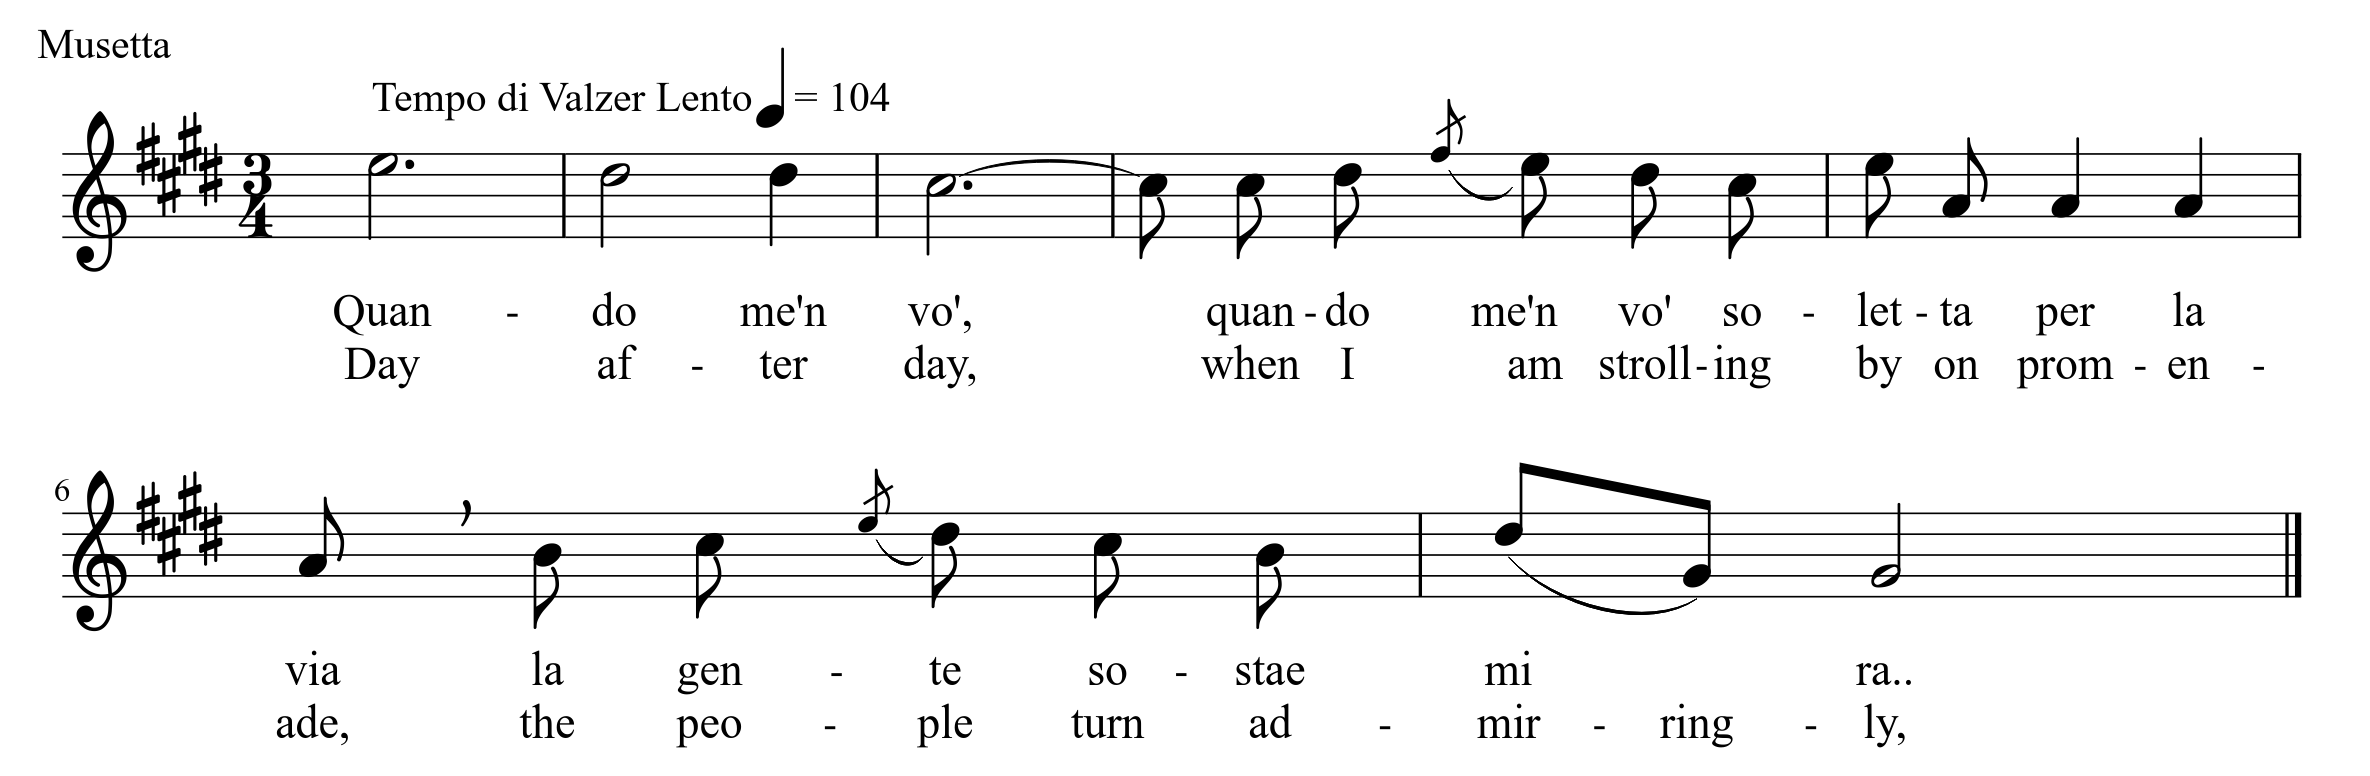
\includegraphics[scale=0.2]{musettatheme}\caption{Musetta's theme}
\label{fig:musettatheme}
\end{figure}

The story, by Henry Murger was published in paperback in 1851 and sold quickly and is autobiographical in nature. The opera attempts to be faithful to the story and the play that followed it. It is a highly sentimental tug at the heart-strings but it reaches out and touches everyone. Compare Puccini and Leoncavallo's treatment of the same theme. 

And of course, if that wasn't enough for Puccini, he continued with \textit{Tosca} (after a play by Victorien Sardou (1831-1908)). The play itself has a torrid history of production and interesting antecedents.

For Puccini, getting around to writing the opera was a long process. There were many premieres of \textit{La Boh\`eme} to attend. Imagine the scene, 5th October 1897. A performance of \textit{La Boh\`eme} in Vienna with Mahler in attendance. Apparently there were too many little children in the Quatier Latin scene and Mahler's laughter, Puccini never forgot.   

\textit{Tosca} has all the ingredients of a tragic opera: Love, betrayal, death between the three key characters; Tosca, Cavaradossi and Scarpia. The scene is Rome, 1800. It does have some of the most intense confrontation scenes in Italian opera and the last scene of Act 1 was well used in Quantum of Solace. The characterisation and the opportunity for highly expressive singing (something 19/20th Century singers must have relished as they propelled themselves to stardom) is there in spades. Perhaps for the tenor (Cavaradossi) it has to be the aria `E lucevan le stelle' early into act III. 

The rest is history. Madame Butterfly - first performed in 1904 and based upon the one act play by David Belasco, itself a dramatisation of a story by John Luther Long, La fanciulla del West, La rondine, a triptych of operas including Gianni Schicchi and of course, Turandot.
  









